\documentclass[runningheads]{llncs}
\usepackage[T1]{fontenc}
\usepackage[utf8]{inputenc}
\usepackage{amsmath,amssymb,booktabs,graphicx,array,multirow}
\usepackage[table]{xcolor}
\definecolor{arcBlue}{HTML}{0F4D92}
\definecolor{arcPale}{HTML}{EDF3FA}
\definecolor{gainGreen}{HTML}{28654A}
\usepackage[hidelinks]{hyperref}
\hypersetup{pdftitle={ARC2-Global: Tangent-Corrected Alignment for Embedding-Index Migration},pdfauthor={Anonymous Author(s)}}
\setlength{\emergencystretch}{2em}
\renewcommand{\topfraction}{0.9}
\renewcommand{\textfraction}{0.1}
\graphicspath{{figures/}}
\newcommand{\method}{ARC2-Global}
\newcommand{\ndcg}{nDCG@10}
\newcommand{\recall}{Recall@100}
\begin{document}
\raggedbottom
\title{ARC2-Global: Tangent-Corrected Alignment\\for Embedding-Index Migration}
\titlerunning{Tangent-Corrected Alignment for Embedding-Index Migration}
\author{Anonymous Author(s)}
\authorrunning{Anonymous Author(s)}
\institute{Anonymous Institution}
\maketitle
\begin{abstract}
Embedding-model upgrades must preserve retrieval quality while document re-encoding proceeds under a limited budget. We propose \method, a compact document adapter that refines centered Procrustes alignment with two ridge-fitted tangent corrections. The updates target cosine-relevant directions and collapse into one affine map, preserving native destination queries without neural mapper training. Across four development collections, two encoder migrations and three anchor-inclusive budgets, \method\ achieves the highest macro \ndcg\ among six evaluated methods. Its gain over Procrustes is 0.0243, with family-adjusted interval [0.0181, 0.0308]; the second correction adds 0.0069. Matched-initialization FiQA/MiniLM controls also favor tangent targeting over chordal and Euclidean residuals, with positive corrected intervals. On prospective TREC-COVID/E5, gains over the evaluated Converter range from 0.2000 to 0.2572. A descriptive comparison across all five collections further shows E5 ARC2 at 25\% coverage exceeding Converter and affine ridge at 75\%. On TREC-COVID/MiniLM, 75\% coverage yields 0.5195 nDCG versus native Full-Y's 0.5203, with the highest Recall@100 point mean among the six adapters. The final 384-to-768-dimensional coefficient matrix occupies 1.13\,MiB, using 114.7 times fewer parameter bytes than the evaluated Converter.
\keywords{Embedding migration \and Vector retrieval \and Representation alignment \and Mixed galleries}
\end{abstract}

\section{Introduction}
\label{sec:introduction}
Embedding-model upgrades create an index-maintenance problem: destination-model queries must remain effective while legacy document vectors are replaced gradually. A staged migration learns from paired embeddings, maps the remaining documents, and replaces these proxies as true destination vectors become available. We seek strong intermediate retrieval with limited destination-document exposure.

The intermediate index must rank true destination embeddings and mapped proxies together. A mapper that works well on a proxy-only gallery can change behavior after true vectors are inserted. Cosine retrieval also depends on direction, whereas coordinate regression spends capacity on radial errors that disappear after normalization. This motivates a directional document adapter that preserves compact inference and searches with the native destination query.

Document conversion and query adaptation bridge embedding spaces~\cite{embeddingconverter,driftadapter}; orthogonal alignment, local alignment and neural regression offer different flexibility~\cite{la2m,simplelinear}. We correct the prediction error that changes direction while retaining one affine document map.

\method\ applies two tangent corrections to centered rectangular Procrustes. Each projects destination error onto the tangent plane at the predicted direction, rescales it to the raw prediction, and fits an affine ridge update. Both updates collapse into one affine map followed by normalization. Native destination queries search true and proxy vectors together; each encoded document replaces its proxy under the same identifier (Fig.~\ref{fig:mechanism}).

The results identify a strong quality--exposure trade-off. On four development collections, the fixed 1,024-pair adapter leads all five baseline configurations in macro \ndcg\ across two migrations and three budgets, gaining 0.0243 over Procrustes. The second correction adds 0.0069 without adding an inference stage. On the prospective TREC-COVID collection, E5 gains over Converter and ridge persist at every budget. Across all five collections, E5 ARC2 at 25\% coverage also exceeds these two alternatives at 75\% in a descriptive comparison. Matched all-paid fitting strengthens MiniLM adaptation by another 0.0596 nDCG at the same paid-document budget.

\noindent\begin{minipage}{\linewidth}
Our contributions are:
\begin{itemize}
  \item \textbf{Directional refinement with affine inference.} Two tangent-residual ridge updates target prediction direction and improve measured development retrieval while retaining one compact document map and native destination queries.
  \item \textbf{Strong quality at matched fitting exposure.} Across two migrations and three paid-document budgets, the four-collection development macro favors \method\ over all five evaluated alternatives. Ablations test the second update and directional targeting under matched initialization; all-paid fitting tests larger supervision.
  \item \textbf{Useful quality at lower document exposure.} A held-collection evaluation confirms E5 gains over Converter and affine ridge at each tested budget. The descriptive 25\%-versus-75\% comparison exposes a useful migration operating point, while mixed-gallery diagnostics explain why adapter choice must be evaluated after native-vector insertion.
\end{itemize}
\end{minipage}

\begin{figure}[t]
\centering
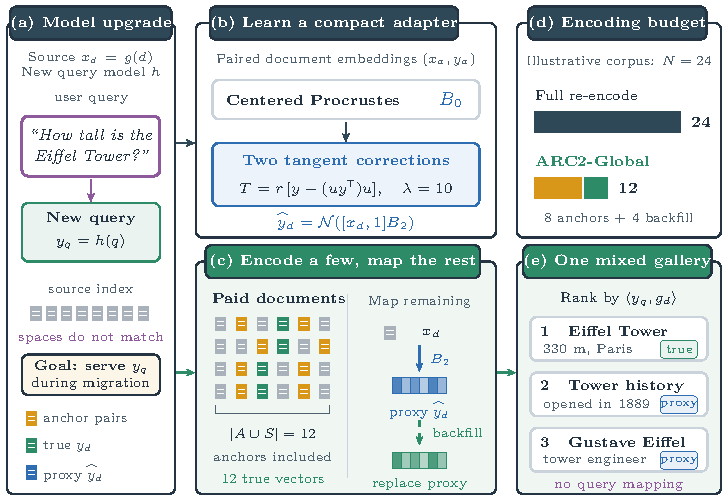
\includegraphics[width=\linewidth]{mechanism.pdf}
\caption{A worked \method\ migration. Paired document vectors train centered Procrustes and two tangent corrections, yielding one affine adapter. Unencoded documents remain searchable through proxies; backfill replaces them with native vectors in the same gallery. The 24-document corpus, eight anchors, four additional encodings and displayed hits are illustrative, not measured retrieval results.}
\label{fig:mechanism}
\end{figure}

\section{Related Work}
\label{sec:related}

\paragraph{Document-side translation and mixed databases.}
Embedding-Converter learns document-side conversion using regression together with global and local similarity losses~\cite{embeddingconverter}.
Yang et al. study integration across embedding models through global alignment and locally fitted isometries, giving the A2M and LA2M approaches~\cite{la2m}.
Their authors' repository also provides the SimpleLinear neural mapper used in our comparison~\cite{simplelinear}.
More recently, Yang and Cao study out-of-distribution translation, multi-model mixing, and chaining, with a hierarchical mixture of experts and residual regularization along target principal directions~\cite{yang2026translation}.
Their localized expert structure addresses broader multi-model integration; our directional target uses the tangent plane at each anchor's current prediction, and both corrections collapse into one global affine map.
FastFill already combines visual feature alignment with uncertainty-based partial backfilling, and shows that replacement can initially reduce retrieval performance~\cite{fastfill2023}.
Building on these migration settings, we study the two-correction affine computation and its relevance-judged text-retrieval behavior under anchor-inclusive encoding budgets.

\paragraph{Compatibility and translation direction.}
Backward-compatible representation learning trains a new encoder to remain usable with previously computed gallery features~\cite{shen2020backward}.
Drift-Adapter instead fits a post-hoc map from new-model queries to an existing legacy index, comparing Procrustes, low-rank affine, and residual neural adapters~\cite{driftadapter}.
Spherical interpolation refines Procrustes-aligned queries through SLERP between old and aligned new query directions~\cite{spherical2026}; ARC2 instead fits tangent ridge updates to document anchors.
ARC2-Global shares the use of paired embeddings and frozen encoders, but maps legacy document vectors into the destination space.
Its evaluation concerns mapped and native destination documents competing as re-encoding progresses.

\paragraph{Geometric alignment and refinement.}
Orthogonal Procrustes provides the classical least-squares alignment underlying our initialization~\cite{schonemann1966procrustes}.
Recent work connects approximate preservation of pairwise inner products to bounds on Procrustes alignment error and demonstrates interoperability across retrieval models~\cite{maystre2025procrustes}.
Unpaired translation pursues a different supervision regime: vec2vec learns translation through a shared latent representation without known correspondences~\cite{jha2025geometry}, while mini-vec2vec combines pseudo-pair construction, Procrustes estimation, and iterative matching and clustering refinements~\cite{dar2025mini}.
GCPA also corrects directional mismatch after Procrustes alignment~\cite{gcpa2026}.
It constructs a shared multi-model universe and trains a residual MLP toward consensus directions with an angular trust penalty.
ARC2 instead targets paired destination documents and regularizes two affine ridge corrections around the current coefficient matrix (Eq.~\ref{eq:current-prior}).
The distinction lies in the destination target, coefficient-space prior and finite affine computation; directional post-alignment correction itself is established.

\paragraph{Retrieval evaluation.}
BEIR emphasizes retrieval across heterogeneous tasks and domains~\cite{beir2021}, while NanoBEIR provides smaller collections suitable for development comparisons~\cite{nanobeir}.
Sentence-BERT, MiniLM, and E5 supply established encoder families and training approaches relevant to our model transitions~\cite{sbert2019,minilm2020,e52022}.
Our evaluation measures judged relevance in the mixed gallery that serves destination queries, separately from vector reconstruction, native-ranking agreement or approximate nearest-neighbor overlap.

\section{\method: Angular Refinement for Mixed Galleries}
\label{sec:method}

\method\ refines one global affine map to combine destination-space proxies
with true destination vectors.

\subsection{Migration Setting and Budget}
\label{sec:setting}

Let a corpus contain $N$ documents with stored, unit-normalized source embeddings
$x_i\in\mathbb{R}^{d_s}$, written as row vectors. The destination encoder produces
unit vectors $y_i\in\mathbb{R}^{d_t}$, but obtaining every $y_i$ requires encoding
the entire corpus again. We seek destination-space document representations
using only a budgeted set of destination document vectors. The dimensions may
differ; our evaluated encoder pairs map $d_s=384$ to $d_t=768$. Queries are encoded
directly by the destination query encoder; the document map aligns with that
existing destination query space.

Let $A$ be the paired anchor set used for fitting and $S$ the set selected for
document replacement. The unique destination-document budget is
\begin{equation}
 b=|A\cup S|,\qquad b=\lfloor\rho N\rfloor .
 \label{eq:budget}
\end{equation}
Anchors consume this budget. Our selection starts with $A$ and fills the
remaining slots from a fixed random document order, skipping duplicates, so
$A\subseteq S$ and $|S|=b$. Larger budgets extend the same order and retain the
same fitted anchors. The principal setting uses $m=|A|=1{,}024$ pairs; an
all-paid-pairs comparison separately fits on every paid pair. Fit uses paired
document vectors without queries or relevance labels. This separates the
amount of fitting supervision from the number of true vectors in the gallery.
The same map serves several replacement budgets; after full replacement,
scores depend entirely on the destination encoder.

\subsection{Centered Rectangular Initialization}
\label{sec:initialization}

A centered Procrustes map supplies a geometric starting point before angular
refinement. Stack the source and destination anchors as
$X_A\in\mathbb{R}^{m\times d_s}$ and
$Y_A\in\mathbb{R}^{m\times d_t}$, with row means $\mu_s$ and $\mu_t$.
Using a thin singular value decomposition, compute
\begin{equation}
 (Y_A-\mathbf{1}\mu_t)^\top(X_A-\mathbf{1}\mu_s)
 =U\Sigma V^\top,\qquad W=UV^\top .
 \label{eq:procrustes}
\end{equation}
Here $W\in\mathbb{R}^{d_t\times d_s}$ is semiorthogonal and accommodates unequal
dimensions. The raw prediction is
$(x-\mu_s)W^\top+\mu_t$.

We expand it into affine coefficients to accumulate corrections without extra
inference stages. With
$p=d_s+1$ and $\widetilde{x}=[x,1]$, define
\begin{equation}
 B_0=\begin{bmatrix}W^\top\\ \mu_t-\mu_sW^\top\end{bmatrix}
 \in\mathbb{R}^{p\times d_t},\qquad
 \widetilde{x}B_0=(x-\mu_s)W^\top+\mu_t .
 \label{eq:affine-init}
\end{equation}
This expansion preserves raw prediction norms, without row normalization
or a fitted scale; those norms enter the correction targets.
The raw affine expansion uses float64 coefficients computed from the
float32 Procrustes means and matrix.

\subsection{Two Tangent-Residual Ridge Corrections}
\label{sec:tangent}

Write $\mathcal N(z)=z/\|z\|_2$ for a nonzero vector $z$.
Cosine retrieval depends on document direction, whereas a raw vector residual
also contains a radial component. We therefore project each anchor target
onto the tangent plane at its current predicted direction. Let
$\widetilde{X}=[X_A,\mathbf{1}]$. At update $t\in\{0,1\}$, for anchor $j$ set
\begin{align}
 z_j^{(t)}&=\widetilde{x}_jB_t,&
 r_j^{(t)}&=\|z_j^{(t)}\|_2,&
 u_j^{(t)}&=z_j^{(t)}/r_j^{(t)},\nonumber\\
 T_j^{(t)}&=r_j^{(t)}\left[y_j-
 \bigl(u_j^{(t)}y_j^\top\bigr)u_j^{(t)}\right].
 \label{eq:tangent-target}
\end{align}
The bracketed term is orthogonal to $u_j^{(t)}$; the norm factor restores raw
prediction coordinates.

The target has a direct cosine-loss interpretation. For a nonzero row
prediction $z$ and unit destination anchor $y_j$, define
$\ell_j(z)=1-y_j\mathcal N(z)^\top$. Differentiation gives
\begin{equation}
 \nabla_z\ell_j(z)=-\frac{y_j-(uy_j^\top)u}{\|z\|_2},
 \qquad T_j^{(t)}=-(r_j^{(t)})^2\nabla_z\ell_j(z_j^{(t)}).
 \label{eq:cosine-target}
\end{equation}
The target is a norm-scaled negative cosine gradient. Shared affine regression
smooths targets across anchors, so fitted row corrections need not be tangent.

One global ridge regression shares these correction targets across anchors.
Stacking their rows into $T^{(t)}$, we solve
\begin{align}
 \Delta_t&=\mathop{\arg\min}_{\Delta\in\mathbb{R}^{p\times d_t}}
 \|\widetilde{X}\Delta-T^{(t)}\|_F^2+\lambda\|\Delta\|_F^2,
 \label{eq:ridge-objective}\\
 &=\widetilde{X}^{\top}
 (\widetilde{X}\widetilde{X}^{\top}+\lambda I_m)^{-1}T^{(t)},
 \qquad B_{t+1}=B_t+\Delta_t .
 \label{eq:tangent-update}
\end{align}
The penalty regularizes the correction, including its intercept. Equivalently,
changing variables to the updated coefficient matrix yields
\begin{equation}
 B_{t+1}=\mathop{\arg\min}_C
 \|\widetilde X C-(\widetilde X B_t+T^{(t)})\|_F^2
 +\lambda\|C-B_t\|_F^2.
 \label{eq:current-prior}
\end{equation}
Unlike zero-centered ridge onto $Y_A$, this penalty retains the current map
while fitting norm-scaled cosine descent targets. We fix $\lambda=10$ and perform
exactly two updates, recomputing targets after the first; the development
ablation in Sect.~\ref{sec:results} measures the second update's contribution.
A Cholesky
factorization is reused across updates. The refined map is unconstrained;
fitting requires paired document vectors and linear solves, with no neural
mapper training.

The norm factor also gives positive global scale equivariance. In exact
arithmetic with nonzero predictions, $T(cB)=cT(B)$ for a common $c>0$.
Linearity of the ridge solve therefore scales each update by $c$; by
induction both accumulated maps scale by $c$, leaving normalized inference
unchanged. This property concerns a common coefficient scale, not arbitrary
per-document changes or guaranteed finite-step cosine improvement.

\begin{table}[t]
\caption{\method\ fitting and gallery construction. All document vectors supplied
to fitting or replacement are unit normalized.}
\label{tab:algorithm}
\centering
\begin{minipage}{0.97\linewidth}
\small
\begin{tabular}{@{}r p{0.89\linewidth}@{}}
\toprule
1 & Form paired anchors $X_A,Y_A$ and augmented design
    $\widetilde{X}=[X_A,\mathbf{1}]$.\\
2 & Compute centered Procrustes and raw affine $B_0$
    using Eqs.~\eqref{eq:procrustes}--\eqref{eq:affine-init}.\\
3 & Factor $\widetilde{X}\widetilde{X}^{\top}+10I_m$ once.\\
4 & For $t=0,1$: compute $T^{(t)}$ from Eq.~\eqref{eq:tangent-target},
    solve Eq.~\eqref{eq:tangent-update}, and accumulate $B_{t+1}$.\\
5 & Store $B_2$; map documents with
    $\widehat{y}_i=\mathcal{N}([x_i,1]B_2)$.\\
6 & Replace rows in $S$ by $y_i$; search with destination query vectors.\\
\bottomrule
\end{tabular}
\end{minipage}
\end{table}

\subsection{Affine Proxies and Mixed Retrieval}
\label{sec:mixed-gallery}

The two corrections collapse into the final coefficient matrix $B_2$.
For each document, compute a proxy
$\widehat{y}_i=\mathcal{N}([x_i,1]B_2)$ and construct
\begin{equation}
 g_i=\begin{cases}
 y_i,&i\in S,\\
 \widehat{y}_i,&i\notin S.
 \end{cases}
 \label{eq:mixed-gallery}
\end{equation}
Every anchor is replaced by its true destination vector. For a unit
destination query $q$, rank by $qg_i^\top$. True and proxy vectors compete in
one score space, so proxy approximation alone does not determine replacement
effects. We use exact
float32 inner products, sorting by descending score and then ascending document
row index for ties; dataset-defined identical query/document IDs are excluded
where specified. Table~\ref{tab:algorithm} summarizes the complete computation.

\subsection{Computation and Storage}
\label{sec:method-cost}

The final mapper has $pd_t$ coefficients regardless of anchor count. For
$384\!\rightarrow\!768$, this is $295{,}680$ float32 values, or $1{,}182{,}720$
bytes ($1.13$\,MiB), including the intercept. This is coefficient storage;
fitting objects, document galleries, and encoder weights are additional.
Application requires one affine multiplication and normalization per document,
with $O(Npd_t)$ arithmetic for a complete proxy gallery.

Fitting cost depends on the solver backend. Beyond the cross-covariance and
rectangular SVD, costing $O(md_sd_t)$ and
$O(d_sd_t\min(d_s,d_t))$, respectively, the reference dual implementation forms an $m\times m$ Gram
matrix in $O(m^2p)$ time, factors it in $O(m^3)$, and spends
$O(m^2d_t+mpd_t)$ per correction. Its Gram storage is $O(m^2)$.
A separately identified primal backend solves
$(\widetilde{X}^{\top}\widetilde{X}+\lambda I_p)\Delta_t=
\widetilde{X}^{\top}T^{(t)}$ instead, with $O(mp^2+p^3)$ construction and
factorization and $O(p^2)$ Gram storage; it supports larger paired sets.
Each primal correction costs $O(mpd_t+p^2d_t)$.
The equations are equivalent in exact arithmetic, while floating-point
rankings can differ near ties. Updates use float64 and the final coefficient
is stored as float32. Finally, $|A\cup S|$ measures logical destination-vector
exposure in cached-vector evaluations. It does not measure physical encoding
work, deployment latency, or end-to-end migration savings.

\section{Experimental Setup}
\label{sec:setup}

We ask three questions: does angular refinement improve fixed-supervision
alignment, how does it compare with other mappers at a matched encoding
budget, and which gains transfer to a prospectively held collection?
All experiments use exact retrieval, isolating representation quality from
approximate-index effects.

\paragraph{Collections and migrations.}
Development uses FiQA (57,638 documents, 500 development queries), NanoNQ
(5,035/50), NanoHotpotQA (5,090/50), and NanoFEVER (4,996/50), drawn from
BEIR and NanoBEIR~\cite{beir2021,nanobeir}. FiQA informed method selection
after its scores were inspected; all four collections are development evidence.
We subsequently fixed a separate confirmation on the BEIR release of
TREC-COVID~\cite{treccovid2020,beir2021}. Its input manifest contains all
171,332 documents and 50 queries. For this study, labels remained
closed until every ranking and endpoint had been sealed and separately
verified. This distinguishes development evidence from the prospective test.
We evaluate two 384-to-768-dimensional migrations:
\texttt{all-MiniLM-L6-v2} to \texttt{all-distilroberta-v1}, and
\texttt{e5-small-v2} to \texttt{e5-base-v2}.\footnote{Pinned maintainer cards:
\href{https://huggingface.co/sentence-transformers/all-MiniLM-L6-v2/blob/1110a243fdf4706b3f48f1d95db1a4f5529b4d41/README.md}{MiniLM},
\href{https://huggingface.co/sentence-transformers/all-distilroberta-v1/blob/842eaed40bee4d61673a81c92d5689a8fed7a09f/README.md}{DistilRoBERTa},
\href{https://huggingface.co/intfloat/e5-small-v2/blob/ffb93f3bd4047442299a41ebb6fa998a38507c52/README.md}{E5-small}, and
\href{https://huggingface.co/intfloat/e5-base-v2/blob/f52bf8ec8c7124536f0efb74aca902b2995e5bcd/README.md}{E5-base}.}
Model revisions and input hashes are pinned. Text encoding uses normalized
float32 vectors, a maximum of 128 tokens, and the E5 query/passage prefixes.

\paragraph{Matched supervision and exposure.}
The main matrix crosses four development collections, two migrations,
three paid-document budgets (25/50/75\%), six methods, and seeds
17, 29, 41, 53, and 67. All methods fit the same ordered 1,024 paired anchors
and replace the same paid document rows. Paid sets contain all anchors and
are nested, with exactly $\lfloor \rho N\rfloor$ unique target document vectors;
the accounting is $|A\cup S|$, including anchors. On the Nano collections and
TREC-COVID, independent seeded streams sample anchors without replacement
and a document permutation; unseen permutation rows fill the budget. FiQA
retains its historical anchor/order arrays. Neither fitting nor selection uses
relevance labels. Paid nonanchor vectors provide replacement only in this
fixed-anchor regime. A separate FiQA experiment holds the 50\% paid set
fixed and compares fitting on 1,024 versus all 28,819 paid pairs.
Development fixed-anchor ARC2 rankings use the float64 dual backend;
all-paid and TREC-COVID fits use the float64 primal backend in
Sect.~\ref{sec:method-cost}. The all-paid study reuses the dual fixed-anchor
comparisons. Both backends implement the same two-update rule.

\paragraph{Matched-target controls.}
An additional FiQA/MiniLM study at 50\% coverage holds $B_0$, the ordered
1,024 anchors, $\lambda=10$, the current-map penalty and two updates fixed.
It replaces the tangent target by either norm-scaled chordal error
$r(y-u)$ or Euclidean error $y-z$, recomputed at each control's own state.
All four arms, including unrefined $B_0$, run in the same Windows environment
(NumPy 2.5.3, SciPy 1.18.1), using float64 dual fitting and the same float32
exact search. This is a separate development measurement.

\paragraph{Comparison methods.}
We retain the full five-baseline panel: centered rectangular Procrustes
(an A2M adaptation); LA2M with 20 source-anchor clusters, local alignment
for clusters with at least two anchors and global fallback for singletons;
SimpleLinear; affine ridge with $\lambda=10$
and a regularized bias; and Embedding-Converter~\cite{la2m,simplelinear,embeddingconverter}.
SimpleLinear uses pinned official code: despite its name, the locked
configuration is a five-layer SELU MLP, trained for the final 50 epochs with
batch size 4,028 and the MSE plus cosine loss, without qrel-based stopping.
Converter is a paper-specification adaptation with a 50,000-update
selection run, batch size 64, and local neighborhood size 100. Paired-vector
validation MAE selects the earliest minimum at 250-update checkpoints;
a fresh fit uses all fitting pairs for that selected length. Unlike the
original retrieval-based validation, this adaptation uses paired-vector MAE
to respect paired-document-only supervision. These are the
declared implementations and training policies, rather than claims to
reproduce every original-paper setting. \method{} remains fixed at two
tangent updates and $\lambda=10$ throughout.

\paragraph{Retrieval and inference.}
Destination queries search a single gallery containing unit-normalized
proxies and paid true vectors, using exact float32 inner products and
top-100 retrieval. Score ties use original document row order; identical
query/document IDs are excluded. Native Full-X and Full-Y use their own
query/document encoders throughout and provide reference operating points.
Our primary metric is graded \ndcg{} with gain $2^{\mathrm{rel}}-1$; auxiliary
\recall{} measures coverage over all
positive judgments, including positives outside a Nano corpus. All queries
count; unjudged documents are nonrelevant. The prospective figure reports both
metrics; a companion Recall table is included in the manuscript-source package.

Each locked analysis uses 20,000 paired query-bootstrap draws after
averaging the five mapping seeds. Development macro effects weight the
24 collection/migration/budget conditions equally and resample queries
within each collection. Within each analysis, the same sampled query indices
are shared across methods, budgets and migrations for that collection.
Saved 99\% percentile intervals give approximate
95\% coverage for the five-comparison family; the ablations have a separate
five-contrast family. The all-paid experiment uses its predeclared
32-contrast family. TREC-COVID has 30 primary contrasts
(five baselines, two migrations, three budgets), with approximately
99.8333\% individual percentile intervals for approximate 95\% family
coverage. Its independent units are the 50 queries. Recall intervals are
nominal 95\% descriptive intervals. An interval touching zero is unresolved.
The matched-target study retains its original four-contrast family, with
98.75\% individual intervals; two MiniLM contrasts are observed and the two
planned E5 contrasts remain pending.
These intervals condition on the five observed mapping seeds and fixed
collections and encoder pairs; development intervals do not adjust for
method selection.\footnote{The accompanying anonymous artifact provides
mapper code, baseline settings, frozen per-query results, raw ranking evidence
and scripts to verify the reported numerical results.}

\section{Results}
\label{sec:results}

\subsection{Broad Retrieval Gains with a Compact Adapter}
% Generated by paper/scripts/build_evidence.py; do not hand-edit.
\begin{table}[t]
\centering
\small
\setlength{\tabcolsep}{4pt}
\caption{Development means at matched 1,024-pair supervision, equally weighting 24 conditions. Differences are ARC2 minus baseline; intervals give approximate 95\% family coverage. Bold/underline mark the best/second unrounded adapter means; blue identifies ARC2.}\label{tab:dev}
\begin{tabular}{lrrrr}
\toprule
Method & nDCG@10 $\uparrow$ & R@100 $\uparrow$ & $\Delta$ nDCG & Family interval \\
\midrule
\rowcolor{arcPale}\textbf{ARC2-Global} & \textbf{0.5275} & \underline{0.8659} & --- & --- \\
Procrustes & \underline{0.5032} & \textbf{0.8661} & \textcolor{gainGreen}{+0.0243} & [+0.0181, +0.0308] \\
LA2M20 & 0.4234 & 0.7758 & \textcolor{gainGreen}{+0.1041} & [+0.0861, +0.1229] \\
SimpleLinear & 0.3554 & 0.6130 & \textcolor{gainGreen}{+0.1721} & [+0.1499, +0.1947] \\
Affine ridge & 0.4318 & 0.7441 & \textcolor{gainGreen}{+0.0957} & [+0.0754, +0.1164] \\
Converter & 0.3663 & 0.7641 & \textcolor{gainGreen}{+0.1612} & [+0.1427, +0.1799] \\
\bottomrule
\end{tabular}
\end{table}

\begin{figure}[t]
  \centering
  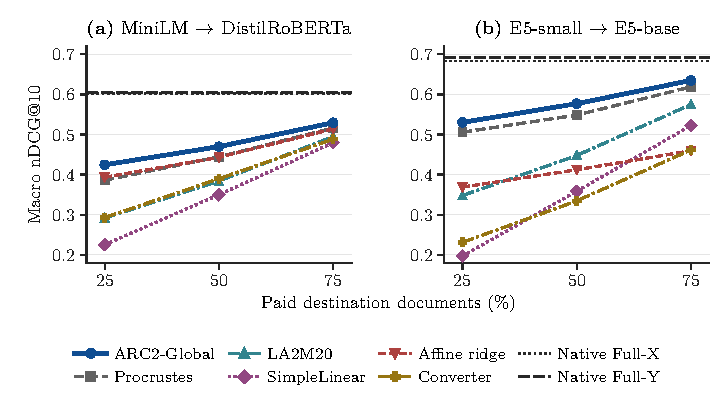
\includegraphics[width=\textwidth]{dev_quality.pdf}
  \caption{Development quality at anchor-inclusive paid-document coverage.
  Points average five seeds and then weight the four collection means equally.
  All six adapters and both native references are retained. Lines connect the
  three measured budgets; they do not imply intermediate measurements.}
  \label{fig:dev-quality}
\end{figure}

\method{} achieves the highest macro \ndcg{} among the six evaluated
methods (Table~\ref{tab:dev}). Its gain over Procrustes is $0.0243$, with
family-adjusted interval $[0.0181,0.0308]$. The effect extends across both
migrations: descriptive pair-wise gains are $0.0257$ for MiniLM and $0.0229$
for E5. Each of the four collection-level macros also favors ARC2 over every
baseline. At the finer condition level, ARC2 leads Procrustes in 23 of 24
point means and every other baseline in all 24. Figure~\ref{fig:dev-quality}
shows the complete budget curves.

The improvement concerns top-ranked relevance: macro Recall is $0.8659$
versus Procrustes' $0.8661$, with descriptive difference interval
$[-0.0049,0.0043]$. The single negative Procrustes nDCG point difference is
FiQA/E5 at 75\% ($-0.0036$). Native Full-X and Full-Y provide the
full-corpus operating context.

\subsection{Directional Targets Add Value without an Inference Stage}
\begin{figure}[t]
  \centering
  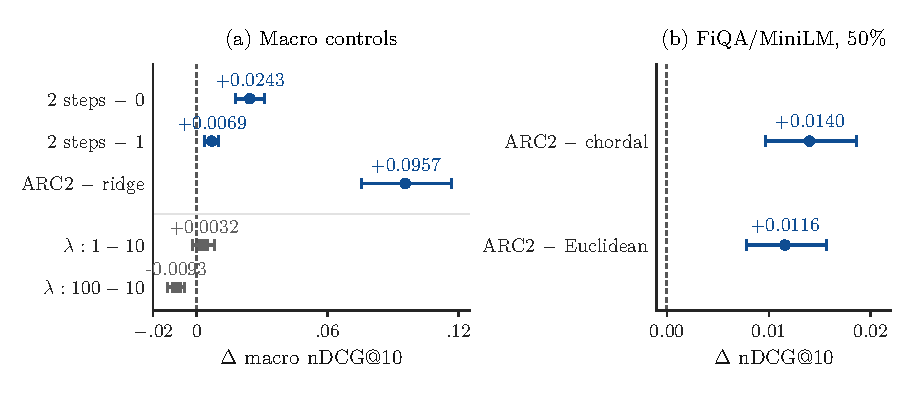
\includegraphics[width=\textwidth]{dev_ablation.pdf}
  \caption{Development mechanism controls. (a) Equal-condition macro effects,
  with saved 99\% intervals for five contrasts. (b) FiQA/MiniLM at 50\%
  coverage: matched-initialization target controls, with 98.75\% intervals
  retaining the original four-contrast family. Panels use separate scales;
  all intervals are shown in full.}
  \label{fig:ablation}
\end{figure}

A second correction adds $0.0069$ macro nDCG beyond one step, with family
interval $[0.0038,0.0100]$. The point gain appears in 22 of 24 conditions
and in each of the five seed-level macros. Both updates retain one affine
inference stage. The complete initialized refinement gains $0.0957$ over
affine ridge (Fig.~\ref{fig:ablation}a), jointly evaluating the target and
alignment prior.

The penalty controls favor moderate regularization. Changing $\lambda$ from
10 to 1 gives $+0.0032$, with an interval crossing zero; changing it to 100
gives $-0.0093$, with a wholly negative interval. The evaluated method keeps
$\lambda=10$ and exactly two corrections.

\paragraph{Tangent targeting improves matched residual controls.}
Holding initialization and supervision fixed isolates an additional benefit
on FiQA/MiniLM (Fig.~\ref{fig:ablation}b). ARC2 reaches $0.3075$ nDCG,
versus $0.2935$ for the norm-scaled chordal control, $0.2959$ for Euclidean
residual refinement and $0.2858$ for unrefined Procrustes. The tangent gains
are $0.0140$ ($[0.0097,0.0186]$) and $0.0116$ ($[0.0078,0.0157]$),
respectively, with both differences positive in all five fixed seed means.
The chordal comparison supports removing the radial target component in this
development configuration. It shares the norm-scaling rule, without imposing
identical later states or equal target norms.

\subsection{Prospective Transfer: Strong E5 Gains and MiniLM Coverage}
% Generated by paper/scripts/build_evidence.py; do not hand-edit.
\begin{table}[t]
\centering
\small
\setlength{\tabcolsep}{4pt}
\caption{Prospective TREC-COVID nDCG@10 (higher is better), averaged over five seeds. $\dagger$: positive ARC2-minus-baseline interval in the 30-contrast family. Unmarked baseline cells are unresolved. Bold/underline rank the six adapters before rounding; native references are separate.}\label{tab:trec}
\begin{tabular}{lrrrrrr}
\toprule
Method & \multicolumn{3}{c}{MiniLM $\rightarrow$ DistilRoBERTa} & \multicolumn{3}{c}{E5-small $\rightarrow$ E5-base} \\
\cmidrule(lr){2-4}\cmidrule(lr){5-7}
 & 25\% & 50\% & 75\% & 25\% & 50\% & 75\% \\
\midrule
\rowcolor{arcPale}\textbf{ARC2-Global} & 0.4619 & 0.5000 & \underline{0.5195} & \underline{0.5628} & \underline{0.5904} & 0.6098 \\
Procrustes & \underline{0.4620} & 0.5046 & \textbf{0.5195} & \textbf{0.5660} & \textbf{0.6067} & \textbf{0.6198} \\
LA2M20 & \textbf{0.4634} & \underline{0.5073} & 0.5186 & 0.5206 & 0.5898 & \underline{0.6188} \\
SimpleLinear & 0.4610 & \textbf{0.5076} & 0.5193 & 0.4299$^{\dagger}$ & 0.5287$^{\dagger}$ & 0.5785 \\
Affine ridge & 0.4322 & 0.4854 & 0.5012$^{\dagger}$ & 0.2986$^{\dagger}$ & 0.3281$^{\dagger}$ & 0.3278$^{\dagger}$ \\
Converter & 0.4224$^{\dagger}$ & 0.4780$^{\dagger}$ & 0.5033 & 0.3056$^{\dagger}$ & 0.3590$^{\dagger}$ & 0.4098$^{\dagger}$ \\
\midrule
Native Full-X & \multicolumn{3}{c}{0.4935 (native)} & \multicolumn{3}{c}{0.6805 (native)} \\
Native Full-Y & \multicolumn{3}{c}{0.5203 (native)} & \multicolumn{3}{c}{0.6421 (native)} \\
\bottomrule
\end{tabular}
\end{table}

\begin{figure}[t]
  \centering
  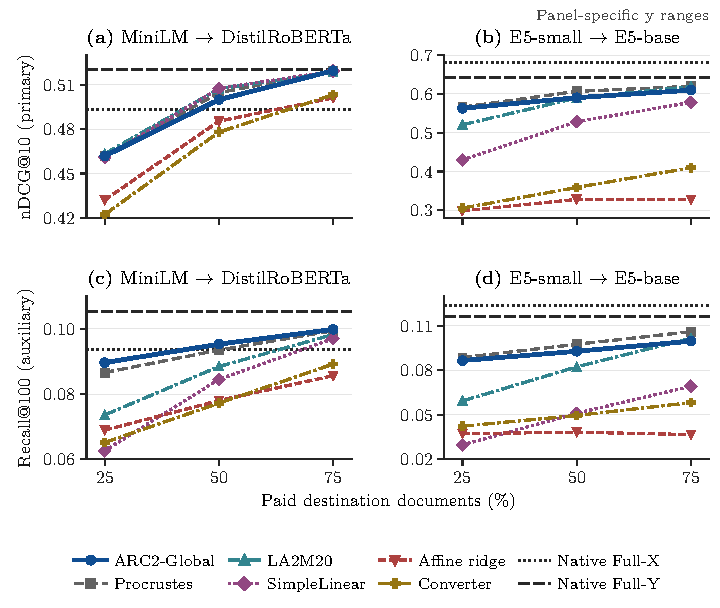
\includegraphics[width=\textwidth]{trec_quality.pdf}
  \caption{Prospective TREC-COVID at fixed 1,024-anchor supervision:
  (a,b) primary nDCG@10; (c,d) auxiliary Recall@100. Points average five
  seeds. All six adapters and native references are shown, with explicitly
  panel-specific vertical ranges. Recall curves are descriptive.}
  \label{fig:trec-quality}
\end{figure}

On the held collection, E5 ARC2 exceeds the evaluated Converter and affine
ridge at \textbf{all three migration budgets}. At 25\% coverage, the
Converter gain is $0.2572$, with family interval $[0.1757,0.3376]$. At 50\%,
ARC2 reaches $0.5904$ nDCG versus Converter's $0.3590$ and ridge's $0.3281$
(Table~\ref{tab:trec}). Across both migrations, the 30-contrast family supports
five improvements over Converter, four over ridge and two over SimpleLinear.
The table marks all eleven supported comparisons.

MiniLM provides a useful partial-migration operating point: at 75\% coverage,
ARC2 reaches $0.5195$ nDCG versus native Full-Y's $0.5203$, while one quarter
of the gallery still uses proxies. Its Recall@100 point mean is the highest
among the six adapters at each budget, reaching $0.0998$ at 75\% versus
native Full-Y's $0.1052$. E5 reaches $0.0997$ Recall at 75\%, versus Full-Y's
$0.1162$ (Fig.~\ref{fig:trec-quality}). These auxiliary results distinguish
coverage at 100 from relevance near the top; proximity in nDCG is not an
equivalence test.

Geometric alignment remains competitive: before rounding, Procrustes has
higher nDCG point means in all six cells, although its MiniLM/75\% difference
is below $0.0001$. All Procrustes and LA2M nDCG family intervals cross zero.
The confirmed advantages therefore concern the evaluated Converter, ridge
and SimpleLinear configurations.

\subsection{Higher E5 Quality at Lower Document Exposure}
% Generated by paper/scripts/build_evidence.py; do not hand-edit.
\begin{table}[t]
\centering
\small
\setlength{\tabcolsep}{2.5pt}
\caption{E5 nDCG: ARC2 at 25\% exceeds Converter and ridge at 75\% on all five collections. Blue identifies ARC2. Proc.: Procrustes; SL: SimpleLinear; native references show full-corpus quality. TREC-COVID is prospective; other rows are development. Cross-budget point comparisons are post-hoc descriptive.}\label{tab:budget-leverage}
\begin{tabular}{lrrrrrrrr}
\toprule
Collection & \multicolumn{3}{c}{25\% coverage} & \multicolumn{3}{c}{75\% coverage} & \multicolumn{2}{c}{Native} \\
\cmidrule(lr){2-4}\cmidrule(lr){5-7}\cmidrule(lr){8-9}
 & ARC2 & Proc. & LA2M20 & SL & Ridge & Conv. & Full-X & Full-Y \\
\midrule
FiQA & \cellcolor{arcPale}\textcolor{arcBlue}{0.2731} & 0.2718 & 0.1416 & 0.2781 & 0.1610 & 0.2095 & 0.3465 & 0.3891 \\
NanoNQ & \cellcolor{arcPale}\textcolor{arcBlue}{0.5071} & 0.4852 & 0.3640 & 0.4839 & 0.4428 & 0.4021 & 0.6595 & 0.6669 \\
NanoHotpotQA & \cellcolor{arcPale}\textcolor{arcBlue}{0.5845} & 0.5512 & 0.3869 & 0.6174 & 0.5053 & 0.5016 & 0.8278 & 0.8193 \\
NanoFEVER & \cellcolor{arcPale}\textcolor{arcBlue}{0.7555} & 0.7147 & 0.4991 & 0.7087 & 0.7290 & 0.7326 & 0.8984 & 0.8963 \\
\midrule \textbf{TREC-COVID} & \cellcolor{arcPale}\textcolor{arcBlue}{0.5628} & 0.5660 & 0.5206 & 0.5785 & 0.3278 & 0.4098 & 0.6805 & 0.6421 \\
\bottomrule
\end{tabular}
\end{table}

A useful budget pattern extends across all five collections
(Table~\ref{tab:budget-leverage}): E5 ARC2 at 25\% coverage exceeds both
Converter and affine ridge at 75\%. On TREC-COVID, the respective nDCG means
are $0.5628$, $0.4098$ and $0.3278$. The advantage is visible even after the
two comparators receive a much larger set of true destination vectors.

This post-hoc descriptive comparison lies outside the matched-budget
inferential family. The table retains geometric alternatives, SimpleLinear
and native references. Physical savings and minimum equal-quality budgets
require separate measurements.

\subsection{Paid Pairs Strengthen MiniLM Adaptation}
% Generated by paper/scripts/build_evidence.py; do not hand-edit.
\begin{table}[t]
\centering
\small
\setlength{\tabcolsep}{4pt}
\caption{FiQA at 50\% coverage. Fixed/All fit 1,024/28,819 pairs; N/R denote nDCG@10/Recall@100. On All-N baseline cells, $\dagger$/$\ddagger$ mark positive/negative ARC2 differences in the 32-contrast family; unmarked comparisons are unresolved. Bold/underline rank matched adapter columns; native rows are references.}\label{tab:allpaid}
\begin{tabular}{lrrrrrr}
\toprule
Method & \multicolumn{3}{c}{MiniLM $\rightarrow$ DistilRoBERTa} & \multicolumn{3}{c}{E5-small $\rightarrow$ E5-base} \\
\cmidrule(lr){2-4}\cmidrule(lr){5-7}
 & Fixed N & All N & All R & Fixed N & All N & All R \\
\midrule
\rowcolor{arcPale}\textbf{ARC2-Global} & \textbf{0.3075} & \underline{0.3671} & \underline{0.6922} & \textbf{0.3116} & 0.2919 & 0.5595 \\
Procrustes & 0.2858 & 0.3334$^{\dagger}$ & 0.6905 & \underline{0.3100} & \textbf{0.3362}$^{\ddagger}$ & \textbf{0.6534} \\
LA2M20 & 0.2377 & 0.3389$^{\dagger}$ & \textbf{0.6950} & 0.2300 & \underline{0.3293}$^{\ddagger}$ & \underline{0.6473} \\
SimpleLinear & 0.2360 & 0.3323$^{\dagger}$ & 0.6778 & 0.1942 & 0.1679$^{\dagger}$ & 0.3618 \\
Affine ridge & \underline{0.2890} & \textbf{0.3673} & 0.6800 & 0.1479 & 0.2270$^{\dagger}$ & 0.4245 \\
Converter & 0.2496 & 0.3258$^{\dagger}$ & 0.6633 & 0.1397 & 0.2625 & 0.5789 \\
\midrule
Native Full-X & \multicolumn{2}{c}{0.3900 (native)} & 0.7002 & \multicolumn{2}{c}{0.3465 (native)} & 0.6453 \\
Native Full-Y & \multicolumn{2}{c}{0.4047 (native)} & 0.7039 & \multicolumn{2}{c}{0.3891 (native)} & 0.6968 \\
\bottomrule
\end{tabular}
\end{table}

Using already-paid pairs improves MiniLM adaptation without increasing the
50\% document budget. ARC2 rises from $0.3075$ to $0.3671$ nDCG, a gain of
$0.0596$ with family interval $[0.0393,0.0806]$. In matched all-paid
comparisons it exceeds Procrustes, LA2M, SimpleLinear and Converter; ridge is
unresolved. Table~\ref{tab:allpaid} makes these family decisions visible.

E5 changes the method ordering: ARC2 trails all-paid Procrustes and LA2M,
exceeds SimpleLinear and ridge, and is unresolved against Converter. Its
fixed-to-all-paid change, $0.3116$ to $0.2919$, is unresolved. Fixed-anchor
MiniLM ARC2 also trails every all-paid baseline in the cross-regime family
comparisons. All-paid fitting retains $\lambda=10$ in the summed objective;
it tests the fixed procedure at larger supervision, rather than isolating
data quantity at a fixed effective penalty.

\paragraph{Evaluate the gallery that will be searched.}
With each fitted map fixed, true-vector replacement raises MiniLM all-paid
nDCG from $0.3510$ to $0.3671$, but lowers E5 from $0.3149$ to $0.2919$.
For E5, Recall falls from $0.6542$ to $0.5595$ and the paid-document share of
top-10 results falls from $0.4916$ to $0.0647$, despite 50\% paid coverage.
These measured replacement effects make mixed-gallery relevance the
appropriate selection criterion: proxy-only quality can favor a different
operating point from the gallery containing native and mapped vectors.

\section{Practical Value of Directional Adaptation}
\label{sec:discussion}
\paragraph{Compact inference with stronger development ranking.}
The 295,680 float32 coefficients occupy 1.13\,MiB, or 114.7 times fewer
parameter bytes than the evaluated Converter. Both corrections are absorbed
into this matrix. Affine ridge has the same coefficient count; refinement
provides the measured quality benefit, while affine mapping provides compactness.

\paragraph{When the adapter is useful.}
ARC2 targets required destination-model queries during staged document
replacement. E5 demonstrates useful quality at limited exposure; MiniLM
benefits from fitting all paid pairs without increasing document coverage.
Procrustes and LA2M remain competitive on the held collection, so deployment
choice should follow encoder-specific mixed-gallery validation. When source
queries remain acceptable, Full-X is also viable: all 24 partial-development
five-seed ARC2 condition means are below it.

\paragraph{Efficiency in the measured units.}
Destination-vector exposure, coefficient storage and the absence of neural
mapper training describe the demonstrated resource advantages. Physical
encoding time, index resources and serving SLOs require deployment measurements.

\section{Conclusion}
\method\ turns two tangent ridge corrections into one compact affine adapter.
Matched-initialization MiniLM controls support its directional target.
It leads five alternatives in development macro nDCG, transfers substantial
E5 gains over Converter and ridge to TREC-COVID, and exposes useful
25\%-versus-75\% quality--coverage operating points. Stronger all-paid
MiniLM adaptation and measured replacement effects further show why
migration should be evaluated in the mixed gallery that serves destination
queries. Angular refinement offers a practical route to budgeted index migration.

\bibliographystyle{splncs04}
\bibliography{references}
\end{document}
